%%%%% Please set the path to 'beamer' directory in your environment %%%%%
\newcommand{\beamerDir}[0]{/mnt/c/Users/atsushi/Documents/workspace/env/Beamer/beamer/beamer/}


%%%%% Load setting %%%%%
\documentclass[aspectratio=169, dvipdfmx, 12pt, compress]{beamer}% dvipdfmxしたい

%%%%% Packages %%%%%
\usepackage{bxdpx-beamer}% dvipdfmxなので必要
\usepackage{pxjahyper}% 日本語で'しおり'したい
\usepackage{tikz}
\usepackage{tcolorbox}
\usetikzlibrary{shapes}
\usepackage{xcolor}
\usepackage[absolute,overlay]{textpos}
\usepackage{adjustbox}
\usepackage{caption}
\usepackage{ifthen}


%%%%% Settings %%%%%
\usetheme[sectionpage=progressbar, subsectionpage=progressbar]{metropolis}
% block style
\metroset{block=fill}
% space between line
\renewcommand{\baselinestretch}{1.3}
% space between item
\newlength{\wideitemsep}
\setlength{\wideitemsep}{0.9\itemsep}
% \addtolength{\wideitemsep}{1.0pt} <- more space
\let\olditem\item
\renewcommand{\item}{\setlength{\itemsep}{\wideitemsep}\olditem}
% frame title
\definecolor{coolblack}{rgb}{0.0, 0.18, 0.39}
\setbeamercolor{frametitle}{bg=coolblack!90,fg=white}
\setbeamerfont{frametitle}{size=\large}
\addtobeamertemplate{frametitle}{}{\vspace{-1em}}
\makeatletter
\setlength{\metropolis@frametitle@padding}{1.4ex}% <- default 2.2 ex
% foot line
\addtobeamertemplate{footline}{}{\vspace{-1em}}
% normal text color
\setbeamercolor{normal text}{fg=black!80}
% progress bar
\definecolor{lightgray}{rgb}{0.83, 0.83, 0.83}
\setbeamercolor{progress bar}{bg=lightgray, fg=coolblack}
\setbeamersize{text margin left=15pt, text margin right=15pt}
% equation font
\usefonttheme{professionalfonts}
% Change standard block width
\addtobeamertemplate{block begin}{%
    \centering
    \begin{columns}\begin{column}{0.9\textwidth}
            \centering
            }{}
            \addtobeamertemplate{block end}{}{\end{column}\end{columns}}
% Change alert block width
\addtobeamertemplate{block alerted begin}{%
    \centering
    \begin{columns}\begin{column}{0.9\textwidth}
            \centering
            }{}
            \addtobeamertemplate{block alerted end}{}{\end{column}\end{columns}}
% Change example block width
\addtobeamertemplate{block example begin}{%
    \centering
    \begin{columns}\begin{column}{0.9\textwidth}
            \centering
            }{}
            \addtobeamertemplate{block example end}{}{\end{column}\end{columns}}
% Itemize color
\setbeamertemplate{itemize item}{\color{black}\scriptsize$\blacksquare$}
\setbeamertemplate{itemize subitem}{\color{black}\scriptsize$-$}
% Simplification  color
\definecolor{cobalt}{rgb}{0.0, 0.28, 0.67}
\setbeamercolor{block title example}{fg=black!80,bg=cobalt!35}
\setbeamercolor{block body example}{fg=black,bg=cobalt!15}
% Definition
\BeforeBeginEnvironment{definition}{
    \setbeamercolor{block title}{use=alerted text, bg=alerted text.fg!70,fg=white}
    \setbeamercolor{block body}{use=alerted text, bg=alerted text.fg!20}
}
\AfterEndEnvironment{definition}{% return to default
    \setbeamercolor{block title}{use=structure,fg=structure.fg,bg=structure.fg!20!bg}
    \setbeamercolor{block body}{parent=normal text,use=block title,bg=block title.bg!50!bg, fg=black}
}
% Theorem
\definecolor{seagreen}{rgb}{0.18, 0.55, 0.34}
\setbeamertemplate{theorems}[numbered]
\BeforeBeginEnvironment{theorem}{
    \setbeamercolor{block title}{fg=black!80,bg=seagreen!40}
    \setbeamercolor{block body}{fg=black,bg=seagreen!15}
}
\AfterEndEnvironment{theorem}{% return to default
    \setbeamercolor{block title}{use=structure,fg=structure.fg,bg=structure.fg!20!bg}
    \setbeamercolor{block body}{parent=normal text,use=block title,bg=block title.bg!50!bg, fg=black}
}
% Lemma
\undef{\lemma}
\newtheorem{lemma}{\translate{Lemma}}
\BeforeBeginEnvironment{lemma}{
    \setbeamercolor{block title}{fg=black!80,bg=seagreen!20}
    \setbeamercolor{block body}{fg=black,bg=seagreen!10}
}
\AfterEndEnvironment{lemma}{% return to default
    \setbeamercolor{block title}{use=structure,fg=structure.fg!80,bg=structure.fg!20!bg}
    \setbeamercolor{block body}{parent=normal text,use=block title,bg=block title.bg!50!bg, fg=black}
}


%%%%% Original Command %%%%%
\newcommand{\subt}[1]{\vspace{-2mm}{\fontsize{10pt}{0cm}\selectfont \textcolor{lightgray}{#1}}\vspace{-1mm}}
\newcommand{\lastpage}[0]{\begin{frame}\begin{textblock*}{1.0\linewidth}(0pt, 50pt)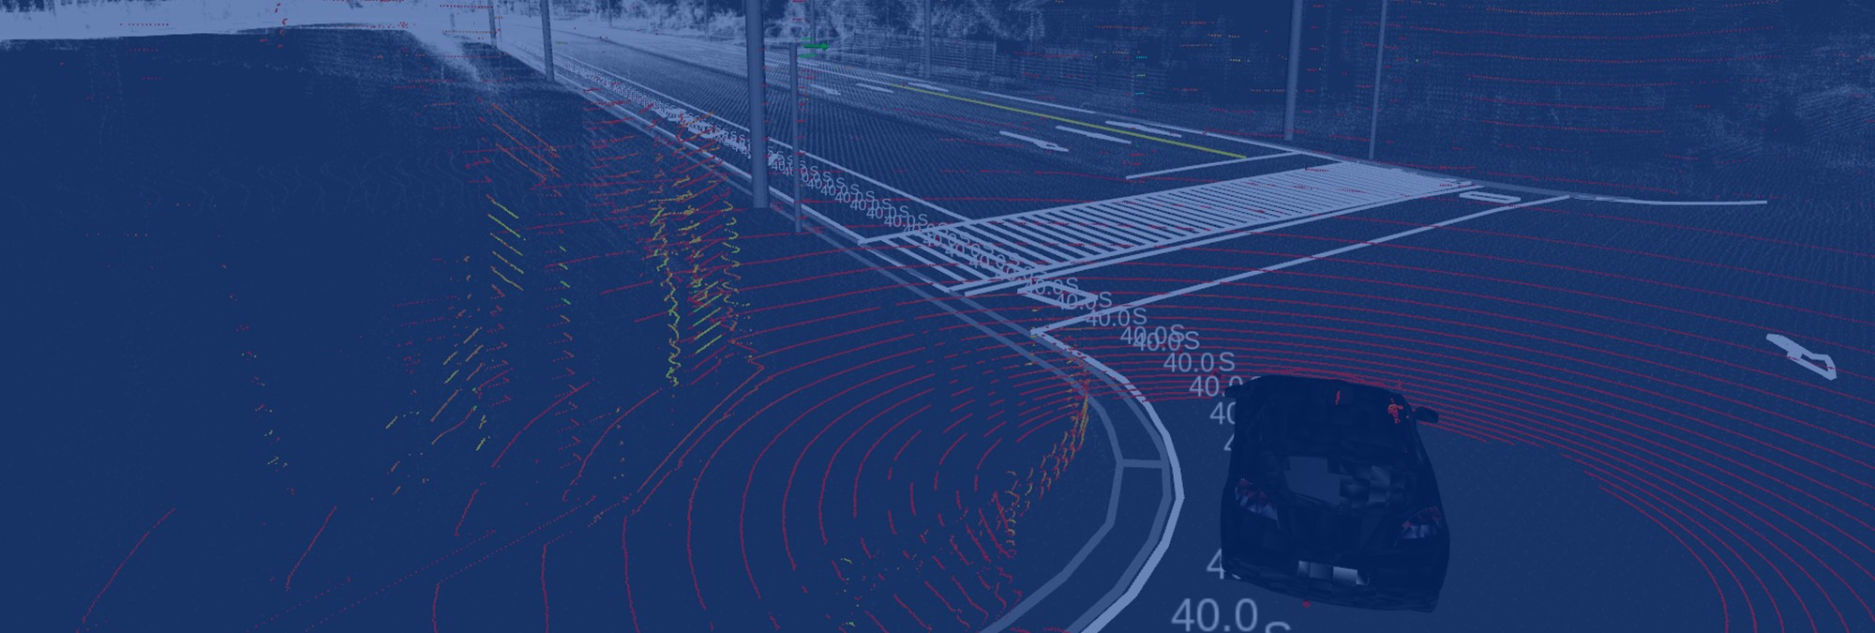
\includegraphics[scale=0.512]{\beamerDir/master_figure/last.pdf}\end{textblock*}\end{frame}}
\newcommand{\todo}[1]{\al{\LARGE\textbf{TODO:} #1}}
\newcommand{\headerheight}[0]{5mm}
\newcommand{\footerheight}[0]{5mm}
\newcommand{\slideheight}[0]{\textheight-\headerheight-\footerheight}
\newcommand{\tabml}[1]{\hspace{-2.1mm}\begin{tabular}{l} #1 \end{tabular}}
\newcommand{\al}[1]{\alert{#1}}
\newcommand{\argempty}[0]{}
\newcommand{\onlyslide}[1]{
    \vspace{\headerheight}
    \begin{minipage}[c][\slideheight][c]{\textwidth}
        #1
    \end{minipage}
}
\newcommand{\onlyimage}[1]{
    \onlyslide{
        \centering
        \begin{columns}
            \begin{column}{\textwidth}
                \centering
                \adjustbox{max width=\textwidth, max height=\slideheight}{
                    \includegraphics{#1}
                }
            \end{column}
        \end{columns}
    }
}
% fit image
\newlength\fitimageht
\newlength\fitotherht
\newsavebox\fitimagebox
\newcommand{\fitimage}[2]{%
    \sbox\fitimagebox{%
        \parbox{\textwidth}{%
            #1\par
        }%
    }%
    \settototalheight{\fitotherht}{%
        \usebox\fitimagebox
    }%
    \setlength\fitimageht{\textheight}%
    \addtolength\fitimageht{-\fitotherht-\headerheight-\footerheight-1\baselineskip}%
    \vspace{\headerheight}
    #1\par
    \centering
    \includegraphics[width=\textwidth,height=\fitimageht,keepaspectratio]{#2}
}
% Simplification
\newcommand{\assume}[1]{
    \begin{exampleblock}{Simplification }
        #1
    \end{exampleblock}
}
% Re-post
\setbeamercolor{RepostBox}{fg=black!50, bg=coolblack!10}
\newcommand{\repost}[1]{
    \vspace{2mm}
    \centering
    \begin{columns}
        \begin{column}{0.86\textwidth}
            \begin{beamercolorbox}[wd=\textwidth, sep=2pt, rounded=true, shadow=true]{RepostBox}
                \begin{tabular}{|p{0.95\textwidth}}
                    {\fontsize{10pt}{10pt}#1}
                \end{tabular}
            \end{beamercolorbox}
        \end{column}
    \end{columns}
}

% equation ballon
\tcbset{
    framebox/.style={
            enhanced,
            boxsep=0pt,       % 箱の上下左右の余白を指定
            colback=white,
            boxrule=1pt,
            colframe=#1
        },
    framebox/.default=red
}
\newcommand{\upbln}[3]{
    \tcboxmath[
        framebox=#2,
        top=0.5ex,bottom=0.5ex,    % 箱の上下の余白を指定
        left=0.5ex,right=0.5ex,    % 箱の左右の余白を指定
        overlay={
                \node[
                    above,
                    rectangle callout,                         % nodeを吹き出しの形に
                    callout absolute pointer={(frame.north)},  % 吹き出しの先端を絶対的に指定
                    fill=#2!20
                ] at ([yshift=2ex]frame.north) {\footnotesize#3};
            }
    ]{#1}
}
\newcommand{\lwbln}[3]{
    \tcboxmath[
        framebox=#2,
        top=0.5ex,bottom=0.5ex,    % 箱の上下の余白を指定
        left=0.5ex,right=0.5ex,    % 箱の左右の余白を指定
        overlay={
                \node[
                    below,
                    rectangle callout,                         % nodeを吹き出しの形に
                    callout absolute pointer={(frame.south)},  % 吹き出しの先端を絶対的に指定
                    fill=#2!20
                ] at ([yshift=-2ex]frame.south) {\footnotesize#3};
            }
    ]{#1}
}
\tcbuselibrary{theorems,skins}



%%%%% Mode %%%%%
% \newcommand{\forme}[1]{#1}
\newcommand{\forme}[1]{}


%%%%% Front Cover %%%%%
\title{Priority-Driven Real-Time Scheduling in ROS 2: Potential and
Challenges}
\subtitle{Real-time And intelliGent Edge computing workshop (RAGE), 2022}
\author{矢野 篤志}
% \date{\today}
\institute[EMBIV]{EMBIV}
\logo{\begin{textblock*}{0.1\linewidth}(2pt, 237pt)
\includegraphics[scale=0.4]{\beamerDir/master_figure/Emb_logo.pdf}\end{textblock*}}


%%%%% Document Start %%%%%
\begin{document}

\maketitle

% \summary{0}{0}
% !TeX root = main.tex


\begin{frame}{提案の概要}
    \begin{itemize}
        \item 優先度駆動型スケジューリングによってROSのリアルタイム性能と予測可能性を大幅に改善できることを主張する
        \item 主張を裏付けるために, 優先度駆動型チェーン考慮スケジューリングに関する我々の研究をレビューし, Apex.AI が開発したオープンソースリファレンスシステムを用いた評価を行う
        \item ROS 2のリアルタイム性能を向上させるために不可欠な以下2つの課題を説明する
        \begin{itemize}
            \item マルチスレッドエグゼキュータ設計
            \item アクセラレータサポート
        \end{itemize}
    \end{itemize}
\end{frame}


\begin{frame}{Outline}
    \setbeamertemplate{section in toc}[sections numbered]
    \scriptsize\tableofcontents[hideallsubsections]
\end{frame}

% !TeX root = main.tex

\section{PRIOR KNOWLEDGE}
\label{sec: prior knowledge}

\begin{frame}{前提知識}
    \begin{itemize}
        \item \ourl{ROS}{https://tier4.atlassian.net/wiki/spaces/EMBIV/pages/2683603071/ROS+Robot+Operating+System}
        \item \ourl{publish/subscribeモデル}{https://tier4.atlassian.net/wiki/spaces/EMBIV/pages/2675048610/Publish+Subscribe}
        \item \ourl{SCHED\_DEADLINE}{https://tier4.atlassian.net/wiki/spaces/EMBIV/pages/2692645566/SCHED+DEADLINE}
        \item \ourl{最大イベント到着曲線}{https://drive.google.com/file/d/1n85X0vDrDm4IDANDP4aUoC0SNnZLAiRN/view?usp=share_link}
        \item \ourl{Casiniらによる先行研究}{https://drive.google.com/file/d/1sHujFqbmgCoJbC6g6KdC7ihua4Jqddju/view?usp=share_link}
    \end{itemize}
\end{frame}

% !TeX root = main.tex

\section{INTRODUCTION}
\label{sec: introduction}

\begin{frame}{}
    \begin{itemize}
        \item ロボット工学のような, 様々な分野の深い専門知識を必要とする学際的で複雑なアプリケーション領域では, 通常, 全ての, あるいはほとんどのソフトウェアをゼロから書くという選択肢はあり得ない
        \item その代わりに, ロボット工学者は, ROSのような一般的なロボット工学フレームワークで容易に利用できる, 標準機能を提供する既存のサードパーティコンポーネントの統合を採用するのが一般的である
        \item その利点は数多く, 簡単に理解できる
        \item 例えば, 複数の最新パス計画アルゴリズムと3D可視化サポートを備えた完全なナビゲーションスタックがたった1回のダウンロードで手に入るなら, なぜ新しいナビゲーションサブシステムを苦労して開発する必要があるか?
    \end{itemize}
\end{frame}

\begin{frame}{}
    \begin{itemize}
        \item 完全なロボットシステムを構築するためには, 多くの相互作用するコンポーネントを統合する必要がある
        \item ROS開発プロセスの分散型オープンソースの性質により, これらのコンポーネントは通常, 必ずしもお互いを知らない複数の独立したコンポーネント開発者によって分離して開発される
        \item 同様に, システムインテグレータは, アプリケーションおよびミッション固有のロジックと「グルーコード」で展開プラットフォーム上で選択したコンポーネントを構成するが, 通常, それぞれのコンポーネント開発者と密接に連携することはない
    \end{itemize}
\end{frame}

\begin{frame}{}
    \begin{itemize}
        \item コンポーネントの統合を可能な限りシンプルに保つために, ROSはコンポーネントの疎結合を可能にする古典的なトピックベースのpublish/subscribeパラダイムを採用している
        \item 概念的には, 各コンポーネントは, 特定のトピックをsubscribeする多数のコールバックを含む「ブラックボックス」として理解できる
        \item 与えられたトピックに関連するメッセージがpublishされるたびに, 全てのsubscribeコールバックが呼び出され, 何らかの計算を実行し, 次に他のトピックに後続のメッセージをpublishすることができ, これがさらにコールバックをトリガするというように, 繰り返す
    \end{itemize}
\end{frame}

\begin{frame}{}
    \begin{itemize}
        \item インテグレータは, あるコンポーネントの「入力コールバック」を別のコンポーネントの「出力トピック」に接続することによってコンポーネントを構成する
        \item ROSシステムは, このように相互接続されたトピックとコールバックの複雑なネットワークを形成し, データ (環境刺激など) は, イベント駆動型の方法でネットワークを通じてcause-effectチェーンに沿って伝播し, インテグレータが望むように透過的にコンポーネント境界を交差させることができる
    \end{itemize}
\end{frame}

\begin{frame}{}
    \begin{itemize}
        \item このようなcause-effectチェーンの典型的な例として, 進路上の障害物を検知して反応する必要のある移動ロボットのセンシング-計算-行動パイプラインが挙げられる
        \item 例えば, ハードウェアドライバコンポーネントがレーザースキャナから新しいサンプルを取得し (cause) , それが複数のマッピング, 座標変換, パス計画, 車輪制御コンポーネントを経て, 最終的に車輪速度の変化 (effect) をもたらす可能性がある
        \item このようなデータ処理のチェーンにおいて, causeからeffectまでの最大レイテンシ時間は, ロボットが正しく機能するために重要な役割を果たすことは明らかであり, また, 安全性を考慮する上でも重要であることが多い
    \end{itemize}
\end{frame}

\begin{frame}{}
    \begin{itemize}
        \item 重要なのは, システムインテグレータにできるだけ多くの展開の選択肢を残し, コンポーネントの再利用の機会を最大化するために, ROSの実行管理層と基礎となるオペレーティングシステムは, 意図的にコンポーネント開発者に公開されないことである
        \item むしろ, ROSの中心的なコールバック抽象化は, コールバック手続きがいつどのようにスケジュールされるか, コールバックの実行がスレッドまたはプロセスにわたってどのように組織されるか, またはネットワーキング層がメッセージの送受信をどのように処理するかを全く意識せずに, 実行から完了までセマンティクスを持つ単なる手続きである
    \end{itemize}
\end{frame}

\begin{frame}{}
    \begin{itemize}
        \item ROSはオープンソースソフトウェアであるため, 原理的にはシステムの実行と通信の挙動を完全に理解し制御することが可能である
        \item このため, リアルタイムシステムの専門家から見れば, ROSにリアルタイムシステム研究でよく知られた技術を導入することは論理的なステップであるように思える可能性がある
        \item しかし, 一見したところ, これを難しくしているハードルがいくつかある
    \end{itemize}
\end{frame}

\begin{frame}{}
    \begin{itemize}
        \item まず第一に, インテグレータに必要な情報が不足している
        \item ほとんどのリアルタイム分析では, 同時実行タスクの数, それらの起動セマンティクスや機能的相互作用, メッセージの到着パターン, 最悪実行時間など, 多くの低レベルシステムの詳細に関する深い知識が前提となっている
        \item ROSコンポーネントは, この種の情報を提供するマニフェストと一緒に来ることはない
        \item さらに悪いことに, リアルタイム分析は, 欠陥のある情報や不完全な情報にうまく対処できない
        \item モデリング目的でサードパーティコンポーネントを手作業でリバースエンジニアリングしているときに, たった一つのミスや見落としがあれば, その取り組み全体を無条件に無効にしてしまうことになりかねない
    \end{itemize}
\end{frame}

\begin{frame}{}
    \begin{itemize}
        \item 第二に, 必要なシステムの詳細をコンポーネントレベルで静的に決定し, 記述することができない
        \item その理由のひとつは, 多くのロボット工学アルゴリズムが, ユースケースやプラットフォーム固有の側面に依存し, 実行時間や起動パターンが大きく変化するためである
        \item 例えば, ビデオストリーム中の物体を識別し, その軌跡を推測する一般的な物体追跡コンポーネントを考えてみよう (例えば, 隣の車線の車など)
        \item この機能の実行時間は, ビデオストリームのフレームレート, 解像度, コーデック, および特定のトラッキングアルゴリズムに関連する他の様々なパラメータを含む, 様々なパラメータに依存する
        \item これらのパラメータは, 一般的なオブジェクトトラッキングコンポーネントの開発者が前もって知っていたり, 固定されていたりするものではない
    \end{itemize}
\end{frame}

\begin{frame}{}
    \begin{itemize}
        \item このようなユースケース特有の情報は, 特定のロボットを構築するインテグレーターにしか分からない
        \item インテグレーターは, 必ずしもオブジェクトトラッキングやリアルタイムシステムの専門家ではないため, 特定の構成を選択した場合の影響を常に予測できるわけではない
        \item したがって, コンポーネントのリソース要求とリアルタイム動作は, 常に特定の展開で使用するという文脈で評価されなければならない
        \item これは, ROSフレームワークの人気の根底にある「ブラックボックス」コンポーネントのモジュール式再利用と相容れるものではない
    \end{itemize}
\end{frame}

\begin{frame}{}
    \begin{itemize}
        \item 最後に, 仮にインテグレータが各コンポーネントについてそれぞれの専門家と議論し, タイミング分析に必要な全ての詳細を入手できたとしても, 第三の根本的な問題が残る
        \item 多くのコンポーネントのリソース要件と性能特性は, 本質的にロボットの動的環境に依存し, したがって時間とともに変化するため, 静的 (最悪のケース) リソース配置は実行不可能なのである
    \end{itemize}
\end{frame}

\begin{frame}{}
    \begin{itemize}
        \item 例えば, 前述の物体追跡コンポーネントと, ランドマークベースの自己位置特定コンポーネントに依存するロボットを再度考えてみよう
        \item 一方, 人口が少ない田舎町よりも, にぎやかな街中を移動する方が, 物体追跡装置の処理時間はずっと長くなる
        \item 一方, 認識可能なランドマークが多い都市部では, ほぼ一様な風景よりも自己位置推定がはるかに容易である可能性が高い
        \item どちらの状況でも十分なリソースを確保するためには, システムインテグレーターは, 不毛の土地からなる賑やかな都市を想定したシステムを用意しなければならない
    \end{itemize}
\end{frame}

\begin{frame}{}
    \begin{itemize}
        \item ロボット工学では, このような悲観的なシステム設計を行うと, すぐに現実的な限界に直面することになる
        \item その代わりに, 実用的で費用対効果の高いシステムを維持するためには, 各コンポーネントのピーク需要の合計ではなく, 予想されるジョイントリソースのピーク需要に対してプロビジョニングを行う必要がある
    \end{itemize}
\end{frame}

\begin{frame}{貢献する}
    \begin{itemize}
        \item これらの課題を克服するために, 我々は, 実行時に動的にタイミングを考慮した方法でROSシステムをプロビジョニングするための自動レイテンシマネージャを使用することを提案する
        \item 具体的には, ROS Live latency manager (ROSLlama) を紹介する
        \item これは, 重要なcause-effectチェーンに沿ったレイテンシを, 非リアルタイム専門家が使いやすく, かつ設定にあまり手間をかけない方法で, 既存のリアルタイム機構を使用して制御することを可能にする
    \end{itemize}
\end{frame}

\begin{frame}{貢献する}
    \begin{itemize}
        \item ROS-Llamaは, 複雑なシステムパラメータをユーザに要求するのではなく, 実行時に必要なパラメータを自動的に推定し, 状況の変化に応じてスケジューリングパラメータを動的に調整することが可能である
        \item もし, 指定されたレイテンシの目標が全て同時に達成できない場合 (例えば, 不利な環境条件による一時的な過負荷が原因) , ROS-Llamaは制御された緩やかなデグレードプロセスを開始し, システムインテグレーターが純粋に宣言的な方法で (すなわち, cause-effectチェーンがどの部品を通過しているかを理解しなくても) cause-effectチェーンの重要性を特定できるようにする
    \end{itemize}
\end{frame}

\begin{frame}{本論文の貢献}
    \begin{itemize}
        \item  ロボティクス領域における動的レイテンシ管理問題を探求し, 実用的なソリューションが満たさなければならない制約と要件を文書化する (第III章)

        \item  ROSのための最初の自動レイテンシマネージャであるROS-Llamaの設計と実装を紹介する (セクションIV)

        \item 標準的な Linux システム上の ROS コンポーネントを用いて, ROS-Llama が移動ロボットのcause-effectチェーンのレイテンシをうまく制御できることを示す評価について報告する (セクションVI)

    \end{itemize}
\end{frame}

\begin{frame}{}
    \begin{itemize}
        \item ROS-Llamaは, 数年にわたる研究とエンジニアリングの努力の結果であり, その間, 我々は多くの課題や技術的な限界に遭遇した
        \item セクションVIIでは, 以下の点を強調する
              \begin{itemize}
                  \item  ROS-Llamaをより効果的かつ正確にするための分析改善の機会
                  \item  ROSとLinuxのプラットフォームには, システムのさらなる改良の妨げとなる大きな限界がある
              \end{itemize}
    \end{itemize}
\end{frame}

% !TeX root = main.tex

\section{PRIORITY-DRIVEN CHAIN-AWARE SCHEDULING}
\label{sec: priority-driven chain-aware scheduling}

\begin{frame}{セクションサマリ}
    \begin{itembox}[l]{\textbf{目的}}
        PiCAS と呼ばれる, ROS 2 用の優先度駆動型のチェーン考慮スケジューリングフレームワークを紹介する
    \end{itembox}
\end{frame}

\begin{frame}{ROS 2 スケジューリングアーキテクチャ再設計の観点}
    チェーンのエンドツーエンドレイテンシを改善するために, 以下2つを考慮して現在の ROS 2 スケジューリングアーキテクチャを再設計する
    \begin{enumerate}
        \item 優先度の高いチェーンを, 優先度の低いチェーンより早く実行する
        \item 各チェーンにおいて, 新しくリリースされたインスタンスが先行インスタンスと同じCPUにスケジューリングされた場合, 新しいインスタンスが実行を開始する前に先行インスタンスの実行を完了する
    \end{enumerate}
\end{frame}

\begin{frame}[label=lemma1]{Lemma 1}
    \hlink{lemma1}{Lemma 1} の2つの条件を満たすスケジューラでは自己干渉が発生しない
    \begin{lemma}[]
        チェーン $\Gamma^{c}:=\left[\tau_{1}, \ldots \tau_{i}, \ldots, \tau_{j}, \ldots, \tau_{N}\right]$ について, $\tau_{i}$, $\tau_{j}$ が同じ CPU 上にある時, 以下2つの条件が満たされれば, 新しいインスタンスが実行を開始する前に, 前のチェーンインスタンスが実行完了する
        \begin{enumerate}
            \item $\tau_{j}$が$\tau_{i}$より高いコールバック優先度を持つ
            \item $\tau_{j}$が$\tau_{i}$のエグゼキュータ以上の優先度を持つエグゼキュータで実行される
        \end{enumerate}
    \end{lemma}
\end{frame}

\forme{
    \begin{frame}{Lemma 1 証明1}
        \fitimage{
            \begin{itemize}
                \item 矛盾によって証明する
                \item 同じCPU上に, 同一チェーンに含まれる $\tau_{i}$, $\tau_{j}$ ($i < j \le N$) が割り当てられているとする
            \end{itemize}
        }{lemma1_proof_sup1}
    \end{frame}

    \begin{frame}{Lemma 1 証明2}
        \begin{itemize}
            \item 新しいチェーンインスタンスが, その前のインスタンスが完了する前に実行を開始するケースは以下3つ:
                  \begin{enumerate}
                      \item $\tau_{i}$ の優先度が $\tau_{j}$ の優先度より高く, $\tau_{i}$ と $\tau_{j}$ が同じエグゼキュータ上に属す
                      \item $\tau_{i}$ は $\tau_{j}$ より優先度が低いが, $\tau_{j}$ より優先度の高いエグゼキュータに属す
                      \item $\tau_{i}$ は $\tau_{j}$ より優先度が高く,  $\tau_{j}$ より優先度の高いエグゼキュータに属す
                  \end{enumerate}
            \item これらは, \hlink{lemma1}{Lemma 1} の少なくとも1つの条件に矛盾する
        \end{itemize}
    \end{frame}

    \begin{frame}{Lemma 1 証明補足 [ケース1の自己干渉例]}
        \fitimage{
            $\tau_{i}$ の優先度が $\tau_{j}$ の優先度より高く, $\tau_{i}$ と $\tau_{j}$ が同じエグゼキュータ上に属す
        }{lemma1_proof_sup2}
    \end{frame}

    \begin{frame}{Lemma 1 証明補足 [ケース1の矛盾]}
        \fitimage{
            $\tau_{i}$ の優先度が $\tau_{j}$ の優先度より高く, $\tau_{i}$ と $\tau_{j}$ が同じエグゼキュータ上に属す
        }{lemma1_proof_sup3}
    \end{frame}

    \begin{frame}{Lemma 1 証明補足 [ケース2の自己干渉例]}
        \fitimage{
            $\tau_{i}$ は $\tau_{j}$ より優先度が低いが, $\tau_{j}$ より優先度の高いエグゼキュータに属す
        }{lemma1_proof_sup4}
    \end{frame}

    \begin{frame}{Lemma 1 証明補足 [ケース2の矛盾]}
        \fitimage{
            $\tau_{i}$ は $\tau_{j}$ より優先度が低いが, $\tau_{j}$ より優先度の高いエグゼキュータに属す
        }{lemma1_proof_sup5}
    \end{frame}

    \begin{frame}{Lemma 1 証明補足 [ケース3の自己干渉例]}
        \fitimage{
            $\tau_{i}$ は $\tau_{j}$ より優先度が高く,  $\tau_{j}$ より優先度の高いエグゼキュータに属す
        }{lemma1_proof_sup6}
    \end{frame}

    \begin{frame}{Lemma 1 証明補足 [ケース3の矛盾]}
        \fitimage{
            $\tau_{i}$ は $\tau_{j}$ より優先度が高く,  $\tau_{j}$ より優先度の高いエグゼキュータに属す
        }{lemma1_proof_sup7}
    \end{frame}
}


\subsection{Strategies for chains running within an executor}
\label{ssec: strategies for chains running within an executor}

\begin{frame}{セクションサマリ}
    \begin{itembox}[l]{\textbf{目的}}
        1つのエグゼキュータ内で実行されるチェーンの戦略について説明する
    \end{itembox}
\end{frame}

\begin{frame}{}
    \fitimage{
        チェーンとコールバックの分類毎にスケジューリング戦略を考える
    }{strategies_classification.png}
\end{frame}

\begin{frame}[label=strategy1]{[戦略 I] 単一チェーンからのレギュラーコールバック}
    戦略 I は $\tau_{j}$ に $\tau_{i}$ よりも高い優先度を与えることで, \hlink{lemma1}{Lemma 1} の最初の条件を満たすようにする
    \begin{block}{戦略 I}
        エグゼキュータが単一のチェーン $\Gamma^{c}=:\left[\tau_{1}, \ldots, \tau_{i}, \ldots, \tau_{j}, \ldots, \tau_{N}\right]$ からのレギュラーコールバックのみを含む場合, それらのコールバックの優先度は, チェーン内の順序とは逆の順序で割り当てる
    \end{block}
\end{frame}

\begin{frame}[label=strategy2]{[戦略 II] 1 つのチェーンからのタイマ/レギュラーコールバック}
    あるチェーンにおいてレギュラーコールバックはタイマコールバックよりも後ろに存在するため, 戦略 II は \hlink{lemma1}{Lemma 1} の最初の条件を満たすようにする
    \begin{block}{戦略 II}
        エグゼキュータに単一チェーン $\Gamma^{c}$ からのタイマ・レギュラーコールバックの両方が含まれる場合, レギュラーコールバックにタイマコールバックよりも高い優先度を与える
        \notes{レギュラーコールバックのスケジューリングは, 戦略 I に従う}
    \end{block}
\end{frame}

\begin{frame}[label=strategy3]{[戦略 III] 複数のチェーンからのレギュラーコールバック}
    戦略 III は \hlink{lemma1}{Lemma 1} の2番目の条件を満たすようにする
    \begin{block}{戦略 III}
        \setlength{\linewidth}{0.98\columnwidth}
        \begin{itemize}
            \item $\pi_{\Gamma^{c}}<\pi_{\Gamma^{c^{\prime}}}$ である2つのチェーン $\Gamma^{c}$, $\Gamma^{c^{\prime}}$ を考える
            \item エグゼキュータに $\Gamma^{c}$ と $\Gamma^{c^{\prime}}$ の両方からのレギュラーコールバックが含まれている場合, $\Gamma^{c^{\prime}}$ の全てのコールバックには, $\Gamma^{c}$ のコールバックよりも高い優先度を割り当てる
                  \notes{各チェーンのコールバックの優先度の割り当ては, 戦略 I に従う}
        \end{itemize}
    \end{block}
\end{frame}

\begin{frame}[label=strategy4]{[戦略 IV] 複数のチェーンからのタイマ/レギュラーコールバック}
    戦略 IV は重要度の高いチェーンインスタンスが重要度の低いインスタンスよりも優先されるようにする
    \begin{block}{戦略 IV}
        優先度の高いチェーンからのタイマコールバックは, 優先度の低いチェーンからのタイマコールバックよりも高い優先度を割り当てる
        \notes{各チェーンは, \hlink{lemma1}{Lemma 1} に準拠するために個別に戦略 II に従う}
    \end{block}
\end{frame}


\subsection{Strategies for chains running across executor}
\label{ssec: strategies for chains running across executor}

\begin{frame}{セクションサマリ}
    \begin{itembox}[l]{\textbf{目的}}
        複数のエグゼキュータ間で実行されるチェーンのスケジューリング戦略について説明する
    \end{itembox}
\end{frame}

\forme{
    \begin{frame}{}
        \begin{itemize}
            \item 各エグゼキュータは 1 つの CPU コアに割り当てられ, OS のプリエンプティブな固定優先度スケジューラによってスケジュールされるため, 複数のエグゼキュータが割り当てられている可能性がある
            \item 各 CPU でチェーンスケジューリングを考慮する必要がある
            \item エグゼキュータは 戦略 I から IV に従うとする
        \end{itemize}
    \end{frame}
}

\begin{frame}{[戦略 V] 1 つの CPU に 1 つのチェーン}
    戦略 V は \hlink{lemma1}{Lemma 1} の 2 番目の条件を満たすようにする
    \begin{block}{戦略 V}
        CPU が 1 つのチェーン $\Gamma^{c}$ からのコールバックのみを持っている場合, $\Gamma^{c}$ の低インデックスコールバック $\tau_{i}$ を含むエグゼキュータは, $\Gamma^{c}$ の高インデックスコールバック $\tau_{j}$ を実行するエグゼキュータ以下の優先度を割り当てる
    \end{block}
\end{frame}

\begin{frame}{[戦略 VI]  1 つの CPU に複数のチェーン}
    戦略 VI はチェーンの優先度を守らせる
    \begin{block}{戦略 VI}
        \setlength{\linewidth}{0.98\columnwidth}
        \begin{itemize}
            \item $\pi_{\Gamma^{c}}<\pi_{\Gamma^{c^{\prime}}}$ である同じ CPU 上の2つのチェーン $\Gamma^{c}$, $\Gamma^{c^{\prime}}$ を考える
            \item CPU に複数のチェーンからのコールバックがある場合, $\Gamma^{c^{\prime}}$ のコールバックを含むエグゼキュータは, $\Gamma^{c}$ のコールバックを含むエグゼキュータ以上の優先度を割り当てる
        \end{itemize}
    \end{block}
\end{frame}


\subsection{Priority assignment of callbacks}
\label{ssec: priority assignment of callbacks}

\begin{frame}{セクションサマリ}
    \begin{itembox}[l]{\textbf{目的}}
        前述のスケジューリング戦略を実現するために, コールバック優先度割り当てアルゴリズムを提案する
    \end{itembox}
\end{frame}

\begin{frame}{コールバック優先度割り当てアルゴリズム全体像}
    \fullimage{alg1}
\end{frame}

\begin{frame}[label=alg1]{コールバック優先度割り当てアルゴリズム補足}
    \fitimage{
        まずチェーンの優先度を考慮し, 次に各チェーン内のコールバックの割り当てる
    }{alg1_sup.jpg}
\end{frame}


\subsection{Chain-aware node allocation scheme}
\label{ssec: chain-aware node allocation scheme}

\begin{frame}{セクションサマリ}
    \begin{itembox}[l]{\textbf{目的}}
        ROS 2 のチェーン考慮ノード割り当てスキームを提案する
    \end{itembox}
\end{frame}

\begin{frame}{提案スキームの方針}
    \begin{itemize}
        \item 提案されたスキームは, 指定されたノードをエグゼキュータに割り当て, 前述のスケジューリング戦略に従いながら, エグゼキュータを使用可能な CPU コアに割り当てる
        \item 提案スキームは, 1つのチェーンに関連する全てのノードを可能な限り同じCPUコアに割り当てることで, チェーン間の干渉を最小化する
    \end{itemize}
\end{frame}

\forme{
    \begin{frame}{提案スキームにおける注意点}
        \begin{itemize}
            \item この割り当て方式はオフラインで実行されるため, 実行時のオーバヘッドは発生しない
            \item また, ノード間の通信はメッセージによって明示的に行われ, どのエグゼキュータを使用しても変わらないため, ノード間のデータ依存関係はノード割り当てに影響されない
        \end{itemize}
    \end{frame}
}

\begin{frame}{フローで使用する表記法}
    \full{
        \begin{table}[tb]
            \adjustbox{max width=\textwidth, max height=\slideheight}{
                \centering\begin{tabular}{|c|l|} \hline
                    $\mathcal{N} $                        & ノードセット                                          \\\hline
                    $\Gamma^{c}$                          & まだ割り当てられていない最高優先度のチェーン          \\\hline
                    $\mathbb{N}$ $(U_{\mathbb{N}} \ge 1)$ & チェーン $\Gamma^c$ のコールバックを含むノードセット  \\\hline
                    $n$ $(n \in \mathbb{N})$              & $\Gamma^c$ の最も低い優先度のコールバックを含むノード \\\hline
                    $e_e$                                 & 空のエグゼキュータ                                    \\\hline
                    $e_m$                                 & 空でないエグゼキュータ                                \\\hline
                    $M$                                   & $e_m$の数                                             \\\hline
                    $P_k$                                 & CPU コア                                              \\\hline
                    $U_{P_k}$                             & CPU コア $P_k$ の利用率                               \\\hline
                    $P$                                   & $P_k$の数                                             \\\hline
                \end{tabular}
            }
        \end{table}
    }
\end{frame}


\begin{frame}{提案スキームの入力}
    提案スキームは以下を入力として受け取る
    \begin{itemize}
        \item \desc{$\mathrm{M}$}{使用するエグゼキュータの最大数}
        \item \desc{$\mathrm{P}$}{使用可能な CPU コアの数}
        \item \desc{$\mathcal{N}$}{割り当てられるノードのセット}
    \end{itemize}
\end{frame}

\begin{frame}{提案スキームの前処理}
    $\mathcal{N}$ 内のノードを, 各ノードに含まれるコールバックの優先度の降順で並べ替える
    \notes{優先度の高いチェーンに関連付けられたノードが最初に割り当てられるようにするため}
\end{frame}

\begin{frame}{提案スキームのフロー全体像}
    \fullimage{proposed_schema.png}
\end{frame}

\begin{frame}{提案スキームを構成する3パート概要}
    \begin{block}{パート A}
        $\mathbb{N}$ を $e_{e}$ に割り当て, $e_{e}$ を実行可能な CPU コアに割り当てる
    \end{block}
    \begin{block}{パート B}
        $e_{e}$ が存在しない場合に, $\mathbb{N}$ に対して実行可能な空でないエグゼキュータ $e_{m}$ を見つける
    \end{block}
    \begin{block}{パート C}
        パートA, Bでエグゼキュータに割り当てられなかった全ての残りのノードを処理する
    \end{block}
\end{frame}

\begin{frame}{共通フロー}
    \fitimage{
        まず $\mathbb{N}$ の利用率が 1 を超えるまで, $\mathcal{N}$ からノードを1つずつフェッチして, ノードのサブセット $\mathbb{N}$ を選択する
    }
    {schema_sup1}
\end{frame}

\begin{frame}{パートAフロー [CPUコアに割り当てられるケース]}
    \fullimage{partA_sup1}
\end{frame}

\begin{frame}{パートAフロー [利用率が1以下のCPUコアが見つからないケース]}
    \fullimage{partA_sup2}
\end{frame}

\begin{frame}{パートAフロー [戦略V, VIを満たすCPUコアが見つからないケース]}
    \fitimage{
        戦略V, VIを満たすCPUコアが見つからない場合, パートCに移行する
    }{partA_sup3}
\end{frame}

\begin{frame}{パートBフロー}
    \fullimage{partB_sup}
\end{frame}

\begin{frame}{パートCフロー}
    \fullimage{partC_sup}
\end{frame}


\forme{
    \subsection{Example of priority-driven chain-aware scheduling}
    \label{ssec: example of priority-driven chain-aware scheduling}

    \begin{frame}{セクションサマリ}
        \begin{itembox}[l]{\textbf{目的}}
            提案するPiCASフレームワークの下で \hlink{exampleChain}{例のチェーンセット} を再実行する
        \end{itembox}
    \end{frame}

    \begin{frame}{PiCASスケジュール結果比較 [単一エグゼキュータ]}
        \fullimage{example_comparison_sched_single}
    \end{frame}

    \begin{frame}{PiCASスケジュール結果比較 [エグゼキュータ2つ]}
        \fullimage{example_comparison_sched_two}
    \end{frame}

    \begin{frame}{PiCASスケジュール結果比較結論}
        PiCASは以下の挙動をする
        \begin{itemize}
            \item 優先度の高いチェーンのコールバックを最初に実行する
            \item 各チェーンの前のチェーンインスタンスは, 新しいチェーンインスタンスの実行開始前に実行を完了する
        \end{itemize}
    \end{frame}

    \begin{frame}{PiCASレイテンシ結果比較}
        \fitimage{
            PiCAS によって両方のチェーンのレイテンシが大幅に改善される
        }{example_picas_latency}
    \end{frame}
}

% !TeX root = main.tex

\section{REAL-TIME SUPPORT FOR MULTI-THREADED EXECUTORS}
\label{sec: real-time support for multi-threaded executors}

\begin{frame}{セクションサマリ}
    \begin{itembox}[l]{\textbf{目的}}
        ROS 2 マルチスレッドエグゼキュータで発生する課題と, 進行中の作業を説明する
    \end{itembox}
\end{frame}

% \begin{frame}{}
%     \begin{itemize}
%         \item ROS 2 はマルチスレッドのエグゼキュータを提供するが, 以前の研究 $[5,6,8]$ ではシングルスレッドのエグゼキュータのみが考慮されていた
%         \item 一般に, マルチスレッド化により, 複数のプロセッサを効果的に利用できるようになり, システムの同時実行性とスループットが向上する
%         \item リアルタイムマルチスレッドの利点は, 自動運転車のコンテキストで実証されている [10]
%         \item また, 図 3 に示すように, ROS 2 のデフォルトのマルチスレッドエグゼキュータは, シングルスレッドのエグゼキュータよりもレイテンシパフォーマンスが優れていることも確認した
%         \item ROS 2 マルチスレッドエグゼキュータのこのような利点にも関わらず,  $\operatorname{ROS} 2$ のマルチスレッドエグゼキュータのタイミング動作を分析および改善するための先行研究はない
%         \item したがって, このセクションでは,
%     \end{itemize}
% \end{frame}

\begin{frame}{マルチスレッドエグゼキュータの分析の困難性}
    マルチスレッドのエグゼキュータでの処理チェーンの分析は以下の理由で困難
    \begin{itemize}
        \item 複数のスレッドにまたがるランタイムコールバックの分散
        \item スレッドの非同期ポーリングポイント
    \end{itemize}
\end{frame}

\begin{frame}{進行中の作業}
    \begin{itemize}
        \item マルチスレッドエグゼキュータを, グローバルスケジューラとしてモデル化し, 従来のノンプリエンプティブグローバルタスクスケジューリング手法を ROS~2 環境に拡張する
        \item PiCAS をマルチスレッドエグゼキュータに拡張して, 優先度に基づくスケジューリングを可能にし, エンドツーエンドレイテンシと予測可能性を向上させる
    \end{itemize}
\end{frame}

\begin{frame}{コールバックグループに関する可能性}
    コールバックグループに関する以下のような問題に関する研究は, ROS 2 でのより効率的なスケジューリングアプローチに繋がる
    \begin{itemize}
        \item コールバックグループが ROS 2 エグゼキュータのタイミング動作にどのように影響するか
        \item 各タイプのチェーンのエンドツーエンドレイテンシを分析的にモデル化する方法
        \item リアルタイムパフォーマンスを向上させるようなコールバックグループ構成
    \end{itemize}
\end{frame}

% !TeX root = main.tex

\section{CHALLENGES WITH REAL-TIME GPUACCELERATION}
\label{sec: challenges with real-time gpuacceleration}

\begin{frame}{セクションサマリ}
    \begin{itembox}[l]{\textbf{目的}}
        GPU アクセラレーションカーネルに依存するアプリケーションの問題に対処する
    \end{itembox}
\end{frame}

\forme{
    \begin{frame}{}
        \begin{itemize}
            \item ROS 2 で設計された多くのアプリケーションは, GPU アクセラレータでのカーネル実行に非同期モデルと非構造化モデルを利用している
            \item これにより, 個々の ROS 2 ノードからの直接的なリソース割り当てとアクセラレータカーネルの呼び出しが促進されるが, これにより, 特に多くのノードが同じアクセラレータリソースを要求する場合に, 予測できないリアルタイムの動作が発生する可能性がある
            \item 自動運転車を含む複雑なソフトウェアスタックに共有アクセラレーターリソースを利用することは, 最新のコンピュータおよびアクセラレーターアーキテクチャでは避けられない
            \item 本論文の進行中の作業は, リソースに制約のあるシステムでリアルタイムの GPU カーネル実行管理を提供することに重点を置いている
        \end{itemize}
    \end{frame}
}


\subsection{Problems with Shared Accelerators}
\label{ssec: problems with shared accelerators}

\begin{frame}{共有アクセラレータの問題点}
    \begin{itemize}
        \item 自動運転スタックの場合, Perception, Localization, Mapping など多くの処理チェーンで GPU ベースのアクセラレータが必要になる
        \item リソースに制約のあるシステムの場合, 優先度の低いチェーンが共有アクセラレーターリソースを既に利用している場合, 優先度の高いチェーンは優先度の逆転により深刻なレイテンシやデッドラインミスが発生する
    \end{itemize}
\end{frame}


\subsection{Maintaining Real-time Support with Accelerators}
\label{ssec: maintaining real-time support with accelerators}

\begin{frame}{従来}
    従来の自動運転車のソフトウェア設計では, 各ノードのコールバックが GPU を直接呼び出してカーネルを実行していた
\end{frame}

\begin{frame}{検討中のアプローチ}
    \begin{block}{検討中のアプローチ}
        \setlength{\linewidth}{0.98\columnwidth}
        \begin{itemize}
            \item 全てのノードからの GPU アクセス要求を処理する GPU サーバとして機能する ROS 2 ノードを利用
            \item GPU サーバアーキテクチャは, リクエストレベルのプリエンプションをサポートする優先度ベースのスケジューリングを採用
            \item リアルタイム空間 GPU マルチタスキング \cite{saha2019stgm, wang2021balancing} と優先度付けされた CUDA ストリーム \cite{xiang2019pipelined} を使用した同時カーネル実行を使用して, リソースの利用率を向上させ, 応答時間を短縮する
        \end{itemize}
    \end{block}
\end{frame}

\begin{frame}{提案アーキテクチャ全体像}
    \fullimage{proposed_arch}
\end{frame}

\begin{frame}{提案アーキテクチャ補足}
    \begin{itemize}
        \item ROS ノードは GPU カーネルスケジューリングノードに, GPU カーネルを特定のデータセットに対して実行するよう要求する
        \item 効率的なゼロコピー IPC メソッドである \ourl{Iceoryx}{https://github.com/eclipse-iceoryx/iceoryx} を使用してデータコピーのレイテンシを最小限に抑える
        \item GPU カーネルスケジューリングノードは, 全ての GPU カーネルの構造を維持し, 対応するチェーンの優先度に従ってカーネルの実行をスケジュールする
        \item OS や GPU ドライバーに任せるのではなく, ソフトウェアスタックで GPU カーネルスケジューリングを処理することで, 特定のチェーンの GPU へのアクセスを細かく制御できる
    \end{itemize}
\end{frame}

% !TeX root = main.tex

\section{CONCLUSION}
\label{sec: conclusion}

\begin{frame}{結論}
    \begin{itemize}
        \item ROS 2のための最初の自動レイテンシマネージャであるROS-Llama を提案した
        \item その設計は, ROSエコシステムの要件と制約の慎重な分析によって形作られている
        \item 我々の評価では, ROS-Llamaは実用的で有益であり, デフォルトのCFSベースラインやSCHED\_RRベースラインのいずれよりも負荷の高い状態でより良いレイテンシ制御を達成することが示された
    \end{itemize}
\end{frame}


\lastpage

\section*{Reference}
\begin{frame}[allowframebreaks]{Reference}
    \beamertemplatetextbibitems
    \bibliographystyle{unsrt}
    \bibliography{\beamerDir/bibtex/master_reference}
\end{frame}

\end{document}
